\newpage
\section{Testen}
\label{test}

Indem technische Geräte und somit auch Software im umfangreichen Maßstab Einzug nehmen in nahezu alle Bereiche des
Lebens ist es wichtig, die Sicherheit, Qualität und Zuverlässigkeit von Software sicherzustellen~\cite[vgl. Introduction]{software-testing}.
Um dies sicherzustellen, sind systematische Tests von Software nötig.
Dabei ist das Ziel, dass die Software bestimmten Anforderungen und Spezifikationen entspricht.
Hierbei werden diverse Techniken und Ansätze verfolgt, die im Folgenden kurz vorgestellt werden.

\subsection{Sichtweisen auf Testsysteme}

Es gibt verschiedene Sichtweisen auf das zu testende System.
Die Sichtweisen können intern oder extern bestimmt sein.
So sind Faktoren wie möglicher Zugriff auf Quellcode oder Architekturdetails des Systems essenziell wichtig, um zu entscheiden, welche Art von Tests angewandt werden sollen.
Es gibt zwei generelle Sichtweisen und eine Mischform.
Das zu testende System wird als Box betrachtet.
Diese Box kann aus verschiedenen Sichten gesehen werden, die im Folgenden näher erläutert werden.
Die Ansätze unterscheiden sich vor allem in den zur Verfügung stehenden Informationen über das System.

\subsubsection{White-Box Testing}

Im White-Box Testing stehen alle Informationen über das System zur Verfügung~\cite[vgl. 1.4.2 Code-Based Testing]{software-testing-craftmans}.
Der Tester hat Zugriff auf Code, Architekturdetails und besitzt Kenntnisse über alle möglichen Details des Systems~\cite[vgl. 1.4.2 Code-Based Testing]{software-testing-craftmans}.
Somit kann der Tester auf alle möglichen Informationen über das System zugreifen und damit seine Tests generieren.
Die erstellten Tests fundieren dann auf einem soliden Niveau, das begründet wird durch das Domänenwissen über das System.
Verschiedene Techniken zur Analyse des Domänenwissens wurden entwickelt, um die Informationen für die Testentwicklung zu nutzen.
In Kapitel~\ref{graphueberdeckung} wird eine dieser Techniken näher untersuchen.

\subsubsection{Black-Box Testing}

Im Black-Box Testing hat der Tester keinen Zugriff auf interne Funktionsweisen der Software.
Schwerpunkt des Testens ist es, dass die Software das tut, was in den Anforderungen gefordert ist~\cite[vgl. Specification-Based Testing]{software-testing-craftmans}.
Da der Quellcode nicht einsehbar ist, muss man sich darauf verlassen, dass die Anforderungen treffend formuliert wurden~\cite[vgl.]{testmanagment}.
Das Black-Box Testing hat einen methodischen Bezug zu Property-based Testing~\cite{property-based-testing}.

\subsubsection{Grey-Box Testing}

Das Grey-Box Testing ist eine Mischform von White-Box und Black-Box Tests~\cite[vgl.]{testmanagment}.
Es sind in dieser Sicht Teile der Software bekannt, aber man hat keinen umfassenden Einblick wie im White-Box Testing.
Es werden sowohl funktionale als auch strukturelle Testansätze verfolgt, je nachdem, wie viel Informationen über das System tatsächlich
verfügbar sind~\cite[vgl.]{graybox}.
Das System wird aus der Sicht des Endbenutzers getestet~\cite[vgl.]{testmanagment}, jedoch mit zusätzlichem Wissen über Teile des internen Aufbaus.

\subsection{Arten von Tests}

Neben verschiedenen Transparenzen auf dem zu testenden System gibt es verschiedene Granularitätsebenen der Tests.
Die Tests können abgeleitet werden von Anforderungen, Spezifikationen, Designartifikaten und dem Programmcode~\cite[vgl. 1.1.1 Testing Levels Based on Software Activity]{software-testing}.
Dabei können verschiedene Level an Tests definiert werden.
Die Level sind eng verbunden mit den Entwicklungsaktivitäten einer Software~\cite[vgl. 1.1.1]{software-testing}.

\begin{figure}[h!]
    \centering
    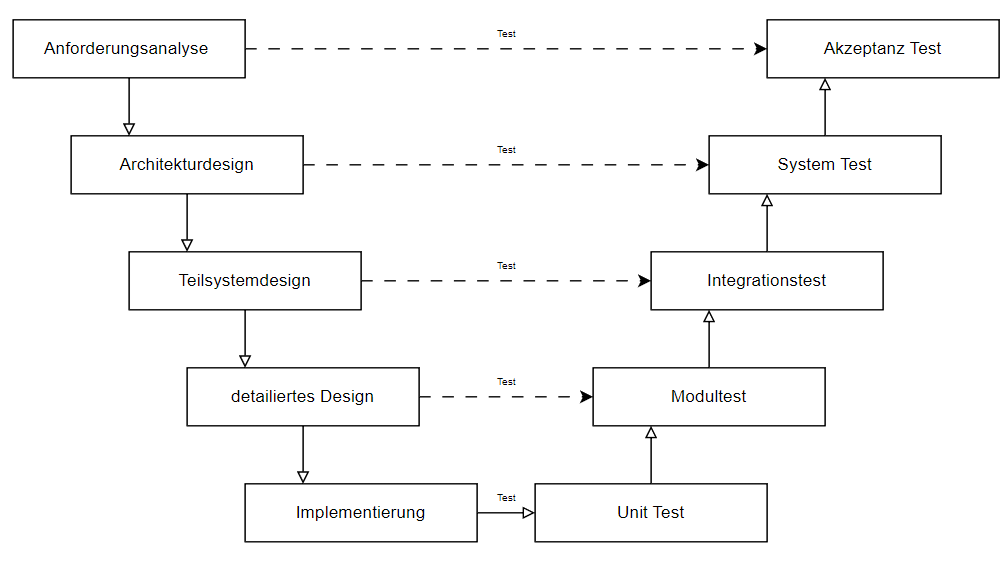
\includegraphics[width=\textwidth,height=\textheight,keepaspectratio]{img/vmodell}
    \caption{Softwareentwicklung und Test-Levels im V-Modell \cite[vgl. Figure 1.2]{software-testing}}
    \label{vmodelltest}
\end{figure}

Die verschiedenen Testebenen sollen schon im Designprozess Beachtung finden, denn die Formulierung von Tests kann dabei helfen, Designfehler zu finden
noch bevor die Software entwickelt wird~\cite[vgl. 1.1.1]{software-testing-ana}.
Die verschiedenen Ebenen der Tests spiegeln auch verschiedene Systemsichten in den Tests.
In Abbildung~\ref{vmodelltest} sind im V-Modell die verschiedenen Schritte der Softwareentwicklung abgebildet.
Dazu passend findet sich im Folgenden die Erklärung der einzelnen Ebenen.

\newpage
\begin{figure}[h!]
    \begin{description}
        \item[Akeptanz Test] - Betrachten der Software hinsichtlich der Anforderungen
        \item[System Test] - Betrachten der Software hinsichtlich der Architektur
        \item[Integrationstest] - Betrachten der Software hinsichtlich der Teilsysteme
        \item[Modultest] - Betrachten der Software hinsichtlich detailliertem Design
        \item[Unit Test] - Betrachten der Software hinsichtlich korrekter Implementierung
    \end{description}\cite[vgl. 1.1.1]{software-testing}
\end{figure}

Im Folgenden wird jede einzelne Testebene präziser betrachtet.
Die Reihenfolge der Betrachtung ist dabei von feingranular zu grobgranular.

\subsubsection{Unit-Tests}

Als feingranularste Testebene ist das Ziel des Unit-Tests, den entwickelten Code zu testen.
Eine einzelne $Unit$ ist in Objekt-Orientierter Programmierung eine Funktion oder Methode~\cite[vgl. Unit Testing]{software-testing-craftmans}.
Der einzelne Unit-Test konzentriert sich dabei auf eine Funktion oder Methode.

\begin{figure}[h!]
    \begin{lstlisting}[language=Python]
        def add(a, b):
            return a + b
    \end{lstlisting}
    \caption{Eine einfache Python-Funktion}
    \label{unitfkt}
\end{figure}

\begin{figure}[h!]
    \begin{lstlisting}[language=Python]
    def test_add_positive():
        self.assertEqual(add(3, 5), 8)

    def test_add_negative():
        self.assertEqual(add(-3, -5), -8)

    def test_add_mixed():
        self.assertEqual(add(5, -3), 2)
    \end{lstlisting}
    \caption{Drei Unit-Tests für die add-Funktion}
    \label{unitfkttest}
\end{figure}

Er prüft, ob die gegebene Einheit bei bekannten Eingaben die erwartete Ausgabe liefert.
Für diese Tests werden häufig Testframeworks genutzt, die bei der Entwicklung und Ausführung der Tests helfen~\cite{software-testing}.
In Abbildung~\ref{unitfkt} wurde eine Funktion definiert und in Abbildung~\ref{unitfkttest} sind drei Unit-Tests mit PyTest~\cite{pytest} definiert.
Die Tests führen verschiedene Methoden aus und prüfen, dass das Ergebnis mit der Erwartung übereinstimmt.
Das $assertEqual$ übernimmt dabei die Auswertung.

\subsubsection{Modul-Test}

Eine Granularitätsebene höher ist der Modul-Test.
Ein Modul ist eine Sammlung von Units~\cite[vgl. S. 6]{software-testing}.
Ziel ist es, die Interoperabilität der einzelnen Units in einem Modul sicherzustellen~\cite[vgl. S. 6]{software-testing}.

\begin{figure}[h!]
    \begin{lstlisting}[language=Python]
        def add(a, b):
            return a + b
        def sub(a, b):
            return a - b
        def mul(a, b):
            return a * b
        def quo(a, b):
            return a / b
    \end{lstlisting}
    \caption{Ein Python Rechenmodul}
    \label{modul}
\end{figure}

In Abbildung~\ref{modul} ist ein Rechenmodul definiert.
Dieses wird getestet, indem verschiedene Funktionen miteinander kombiniert werden und dann geprüft wird, ob Erwartung und Ergebnis übereinstimmen.
Ein Modul-Test für das Modul aus Abbildung~\ref{modul} ist in Abbildung~\ref{modultest} definiert.

\begin{figure}[h!]
    \begin{lstlisting}[language=Python]
    def test_rechenmodul():
        testResult = (mul(add(2,3), sub(3,2)))
        self.assertEqual(testResult, 5)
    \end{lstlisting}
    \caption{Ein Modul-Test}
    \label{modultest}
\end{figure}

Es ist anzumerken, dass die Interoperabilität im Modul-Test nur innerhalb eines Moduls getestet wird~\cite[vgl. S. 6]{software-testing}.

\subsubsection{Integrations-Test}

Die Integrations-Tests übernehmen das Testen von Interoperabilität zwischen verschiedenen Modulen~\cite[vgl. S. 7]{software-testing}.
Es wird davon ausgegangen, dass die einzelnen Module zuvor korrekt getestet worden sind und die einzelnen Module korrekt arbeiten~\cite[vgl. S. 7]{software-testing}.
Testobjekte sind die Schnittstellen der einzelnen Module und somit auch die Kommunikation zwischen den Modulen.

\begin{figure}[h!]
    \begin{lstlisting}[language=Python]
def newUser(name, gb, email):
    pw = generateRandomPw()
    return new User(name, gb, email, pw)
    \end{lstlisting}
    \caption{Modul 1}
    \label{modul1}
\end{figure}

\begin{figure}[h!]
    \begin{lstlisting}[language=Python]
def saveUser(User user):
    db.save(user)
def getUser(name):
    db.findUser(name)
    \end{lstlisting}
    \caption{Modul 2}
    \label{modul2}
\end{figure}

In Abbildung~\ref{modul1} ist ein Modul definiert, das einen neuen Nutzer erstellen kann.
Abbildung~\ref{modul2} definiert ein Modul, das Nutzer speichern und finden kann.
Ein Integrations-Test beider Module sollte testen, ob ein neu angelegter Nutzer ordentlich gespeichert wird und ob die dabei zugewiesenen Daten auch passend bleiben.
In Abbildung~\ref{integtest} ist ein solcher Modultest zu finden.

\begin{figure}[h!]
    \begin{lstlisting}[language=Python]
def testAddNewUserAndSaveUserAndGetUser():
        user = newUser("Peter", "01.04.1980", "p@test.de")
        saveUser(user)
        self.assertEqual(getUser("Peter"), user)
    \end{lstlisting}
    \caption{Integrations-Test zwischen Modul 1 und Modul 2}
    \label{integtest}
\end{figure}

Im Kontext dieser Arbeit gilt es zu untersuchen, wie Integrations-Tests automatisiert für GraphQL erstellt werden können.
Hinter jedem verschiedenen Typen von GraphQL steckt ein Resolver, welcher als ein eigenes Modul gesehen werden kann.
Die Interoperabilität dieser Module gilt es im Folgenden automatisiert zu testen.

\subsubsection{System-Test}

Um zu testen, ob nicht nur einzelne Teile des Systems gut miteinander funktionieren, sondern auch das ganze System als
Solches, werden die System-Tests genutzt~\cite[vgl. S. 6]{software-testing}.
Die Tests werden auf Grundlage der Spezifikation des Systems erstellt.
Es wird davon ausgegangen, dass die einzelnen Module hier wie erwartet funktionieren.
Im Vordergrund dieser Testebene steht, dass die Software die Spezifikation, also die Erwartungen an sich, erfüllt.

\subsubsection{Akzeptanz-Test}

Die finale Ebene des Testprozesses ist der Akzeptanz-Test.
Auf dieser Ebene wird die Software aus Sicht des Endnutzers geprüft, oft ist der Endnutzer auch Teil dieses Prozesses~\cite[vgl. S.6]{software-testing}.
Ziel ist es, zu verifizieren, dass die Analyse und Umsetzung des Problems erfolgreich ist und der Nutzer mit der entwickelten Lösung
zufrieden ist~\cite[vgl. S.6]{software-testing}.

\subsection{Testabdeckung}
\label{abdeck}

Bisher ungeklärt ist, wann ausreichend getestet wurde und ob überhaupt genügend getestet werden kann.
Hierzu werden die formalen Abdeckungskriterien eingeführt, wie sie in~\cite{software-testing} definiert sind.
Mithilfe dieser Abdeckungskriterien wird es möglich, sinnvolle Testfälle zu entwickeln und zu entscheiden, wann ausreichend getestet wurde.
Die Notwendigkeiten für solche Abdeckungskriterien zeigt sich schnell.
Ein Ausprobieren aller Kombinationen ist in der heutigen Zeit unmöglich.
Als Beispiel sei hier eine simple Addition von 2 64-bit Integer genannt.
Für eine komplette Testung dieser Addition gibt es $2^{64}$ Kombinationen.
Mit einem 3GHz-Prozessor wäre eine vollständige Testung nach etwa 69 Tagen erledigt.
Betrachtet man einen Java-Compiler, so ist der Eingaberaum von Programmen, die zum Test stehen, effektiv unendlich und somit nicht testbar~\cite[vgl. 1.3 Coverage Criteria for Testing]{software-testing}.

\subsubsection{Abdeckungskriterien}

Da ein vollständiges Testen, also ein Ausprobieren aller Möglichkeiten, unmöglich ist, müssen Kriterien geschaffen werden, die eine hinreichende Testqualität zusichern.
Hierfür werden die Abdeckungskriterien eingeführt.
Diese liefern einen Ansatz, der dabei hilft, sinnvolle Tests zu entwickeln und abzuschätzen, wann ausreichend getestet wurde.
Im Folgenden werden die Abdeckungskriterien auch als Testanforderungen~\cite[vgl. 1.3 Coverage Criteria for Testing]{software-testing} gesehen.

\begin{definition}
    Eine Testanforderung ist ein spezifisches Element eines Softwareartifkates das einen Testfall erfüllen muss~\cite[Def. 1.20]{software-testing}.
    \label{tr}
\end{definition}

Dabei ist ein Abdeckungskriterium erfüllt, wenn alle seine Testanforderungen erfüllt sind.

\begin{definition}
    Ein Abdeckungskriterium ist eine Regel oder eine Sammlung von Regeln, die Testanforderungen an eine Menge von Testfällen stellen~\cite[Def. 1.21]{software-testing}.
\end{definition}

Um eine Aussage darüber zu machen, wie gut eine Menge an Tests das Abdeckungskriterium umsetzt, wird die Abdeckung eingeführt.
Einerseits ist es manchmal sehr schwierig, ein Abdeckungskriterium vollständig zu erreichen, andererseits kann dann gemessen werden, ob das Kriterium erfüllt wurde~\cite[vgl. S. 18]{software-testing}.
Durch die Definition~\ref{abd} wird messbar, wie gut eine Menge an Tests das Abdeckungskriterium umsetzt und ob das Kriterium erfüllt ist.

\begin{definition}
    Gegeben sei eine Menge an Testanforderungen $TR$ für ein Abdeckungskriterium $C$. 
    Eine Menge an Testfällen $T$ erfüllt $C$ wenn gilt, 
    dass für jede Testanforderung mindestens ein Test existiert der diese Testanforderung erfüllt~\cite[vgl. Def. 1.22]{software-testing}.
    \label{abd}
\end{definition}

Es gibt diverse Abdeckungskriterien, die auf verschiedenen Annahmen beruhen.
Ist das Ziel, dass alle Entscheidungen in einem Programm abgedeckt sein sollen (Branch-Coverage), so führt jede Entscheidung zu zwei
Testanforderungen, eine Anforderung für den positiven und eine für den negativen Entscheidungsfall~\cite[vgl. S. 17]{software-testing}.
Soll jede Methode mindestens einmal aufgerufen werden (Call-Coverage), so führt jede Methode zu einer Testanforderung, um diese Methode abzudecken~\cite[vgl. S. 17]{software-testing}
Im folgenden Kapitel~\ref{graphueberdeckung} werden Abdeckungskriterien speziell für Graphen eingeführt.